%!TEX program = xelatex
%!TEX encoding = UTF-8

\documentclass[fangfont=STFANGSO.TTF,heifont=YaHeiConsolas.ttf]{zju-proposal}
\usepackage{url}
\usepackage{pdfpages}
\title{动态因子模型在高维数据中的应用(有监督的动态因子模型预测)}{浙江大学本科生毕业论文(设计)}
\author{汪利军}{3140105707}
\grade{14 级}{统计学}
\mentor{张荣茂}
\school{数学科学学院}
%\myfonts{STFANGSO.TTF}{YaHeiConsolas.ttf}

\usepackage{amsmath}
\usepackage{amssymb}
\usepackage{bm}
\usepackage{amsfonts}

%% custom commands (optional)
%% which might save time via simpler commands
\newcommand\e{\mathbf e}
\renewcommand\v{\mathbf v}
\newcommand\g{\mathbf g}
\renewcommand\m{\mathbf m}
\newcommand\z{\mathbf z}


%% cal style
\renewcommand\L{{\cal L}}
\newcommand\N{{\cal N}}
\renewcommand\U{{\cal U}}


%% mathbf style
\newcommand\F{\mathbf F}
\renewcommand\H{\mathbf H}
\newcommand\I{\mathbf I}
\newcommand\J{\mathbf J}
\renewcommand\M{\mathbf M}
\newcommand\R{\mathbf R}
\newcommand\V{\mathbf V}
\newcommand\W{\mathbf W}
\newcommand\X{\mathbf X}
\newcommand\Z{\mathbf Z}

%% boldsymbol for Greek alphabet and Arabic numberals
\newcommand\zero{{\boldsymbol 0}}

\newcommand\bfvarepsilon{{\boldsymbol \varepsilon}}
\newcommand\bfrho{{\boldsymbol \rho}}
\newcommand\bftheta{{\boldsymbol \theta}}
\newcommand\bflambda{{\boldsymbol \lambda}}
\newcommand\bfLambda{{\boldsymbol \Lambda}}
\newcommand\bfOmega{{\boldsymbol \Omega}}
\newcommand\bfGamma{{\boldsymbol \Gamma}}
\newcommand\bfSigma{{\boldsymbol \Sigma}}
\newcommand\bfPsi{{\boldsymbol \Psi}}
\newcommand\bfxi{{\boldsymbol \xi}}
\newcommand\bfXi{{\boldsymbol \Xi}}


%% mathrm style
\newcommand\tr{\mathrm{tr}}
\renewcommand\vec{\mathrm{vec}}
\newcommand\diag{\mathrm{diag}}
\newcommand\pd{\mathrm{p.d.}}
\newcommand\gmm{\mathrm{gmm}}
\newcommand\iid{\mathrm{iid}}


%% some shorter commands for longer commands
\newcommand\toinf{\rightarrow\infty}
\newcommand\pto{\overset{p}{\rightarrow}}
\newcommand\dto{\overset{d}{\rightarrow}}
\newcommand{\bsum}[2]{\sum\limits_{#1}^{#2}}
\newcommand{\ssum}[2]{\sum_{#1}^{#2}}
\newcommand{\abs}[1]{\vert #1\vert}
\newcommand{\norm}[1]{\Vert #1\Vert}

%% Roman numberals
\newcommand{\rmnum}[1]{\romannumeral #1}
\newcommand{\Rmnum}[1]{\expandafter\@slowromancap\romannumeral #1@}
\begin{document}
	\makecover
	\begin{refsection}
	\addtocontents{toc}{\protect\contentsline{guide}{\protect\numberline{}指导教师对文献综述和开题报告具体要求}{}}
	\thispagestyle{guidepage}
	\end{refsection}
	%\setcounter{page}{-3}
	\tableofcontents
	
	\begin{refsection}	
	\chapter{文献综述(仿宋3号加黑)}
\section{背景介绍(顶格、小三号仿宋加黑)}
(小四号或12磅仿宋,1.5倍行距)

\subsection{那些酷炫的论文(节的标题、四号仿宋加黑)}
(仿宋小四号或12磅,1.5倍行距)
\subsubsection{那些大牛作者们(顶格、四号仿宋加黑)}
(小四号或12磅仿宋,1.5倍行距)

{\bfseries TODO:}

图、表标题均采用五号宋体加粗。表格中文字采用5号宋体,行距为单倍行间距。图、表与下文空一行
\section{国内外研究现状}
\subsection{研究方向及进展}
\subsection{存在问题}
\section{研究展望}

\lipsum[1]

\parencite{small}

\printbibliography[heading=secbib]
	\end{refsection}
	
	\begin{refsection}
	\chapter{开题报告(仿宋3号加黑)}

\section{问题提出的背景(顶格、小三号仿宋加黑)}

\subsection{背景介绍(节的标题、四号仿宋加黑)}

\subsubsection{那些不为人知的故事(顶格、四号仿宋加黑)}

\subsection{本研究的意义和目的}

\section{论文的主要内容和技术路线}

\subsection{主要研究内容}

\subsection{技术路线}

\subsection{可行性分析}

\section{研究计划进度安排及预期目标}

\subsection{进度安排}

\subsection{预期目标}

\section{参考文献}
	\end{refsection}
	\begin{refsection}
	\chapter{外文翻译(仿宋3号加黑)}

(正文格式与文献综述部分相同)

\lipsum[3-7]
	\end{refsection}
	\chapter{外文原文(仿宋3号加黑)}

\lipsum[11-21]
	

%	\printbibliography

	%\setboolean{@twoside}{false}
%	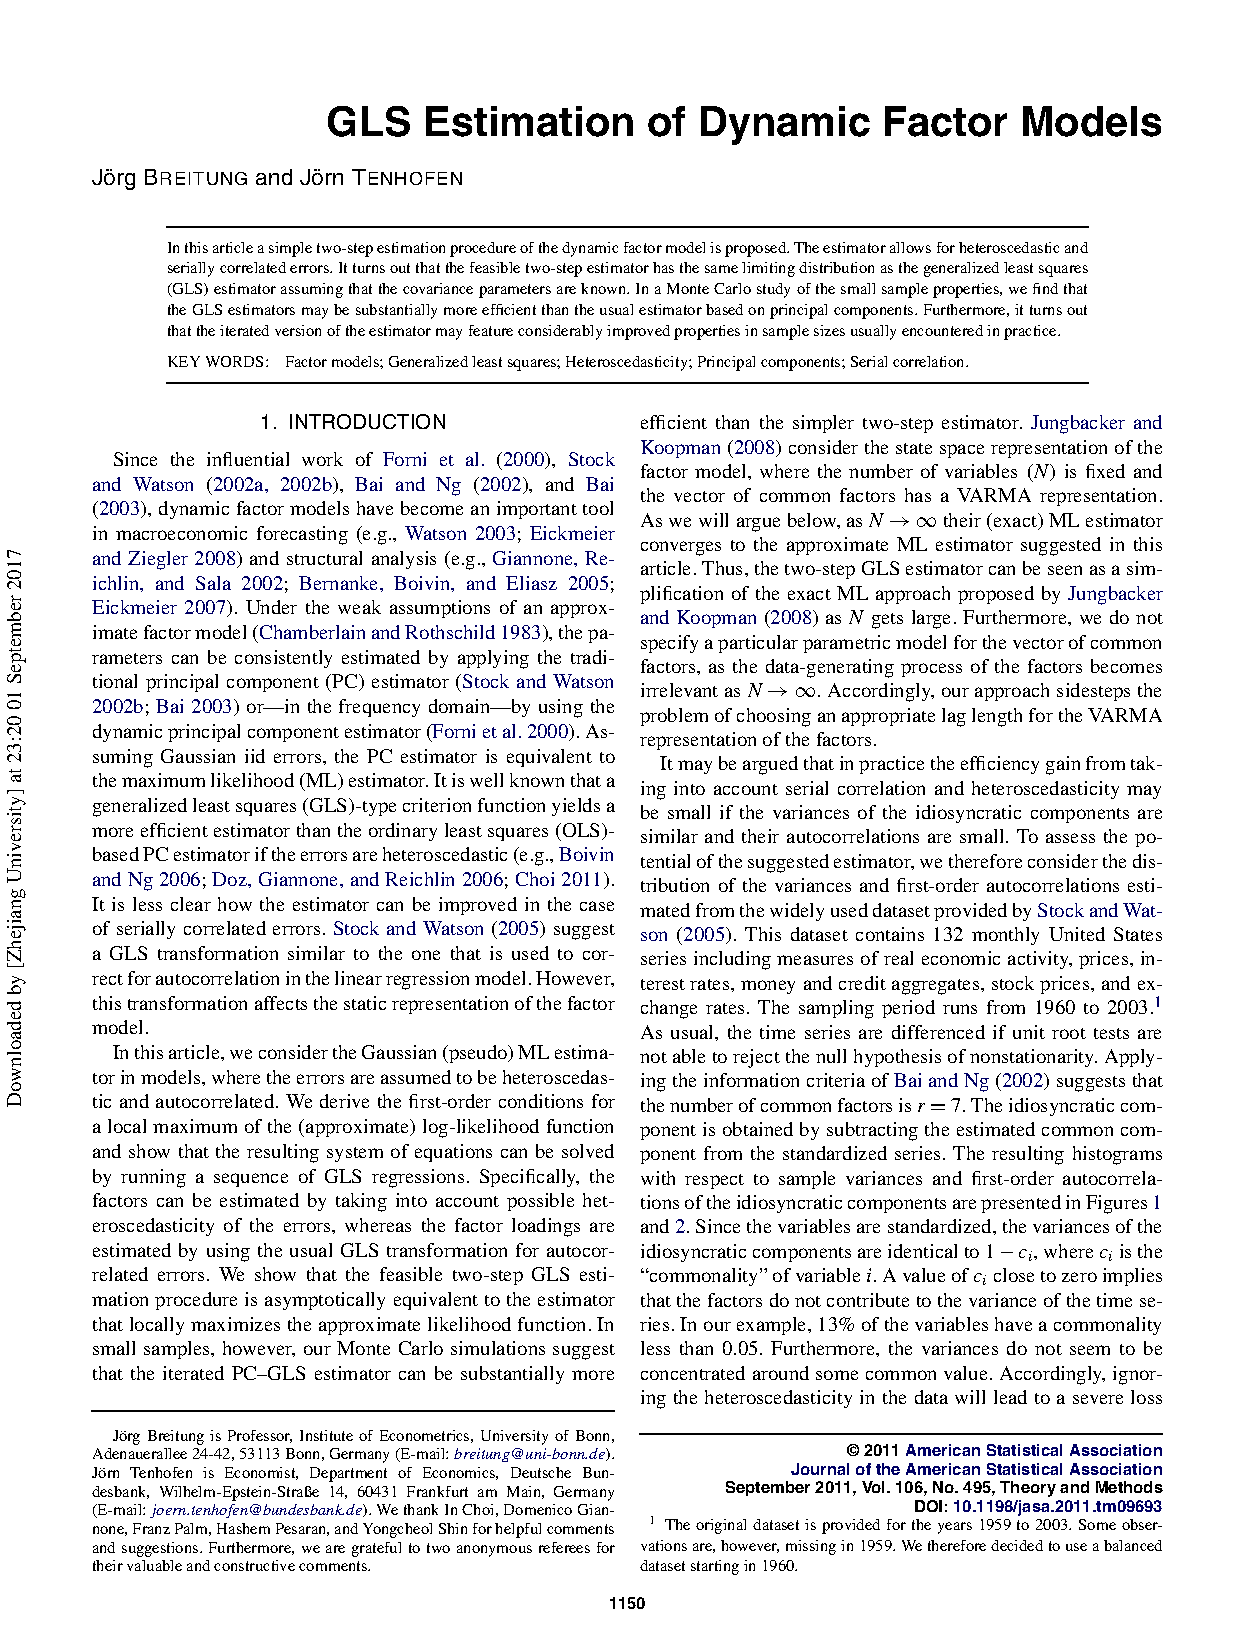
\includepdf[fitpaper= true, pages=-,pagecommand={\thispagestyle{}}]{gls-original-2.pdf}
	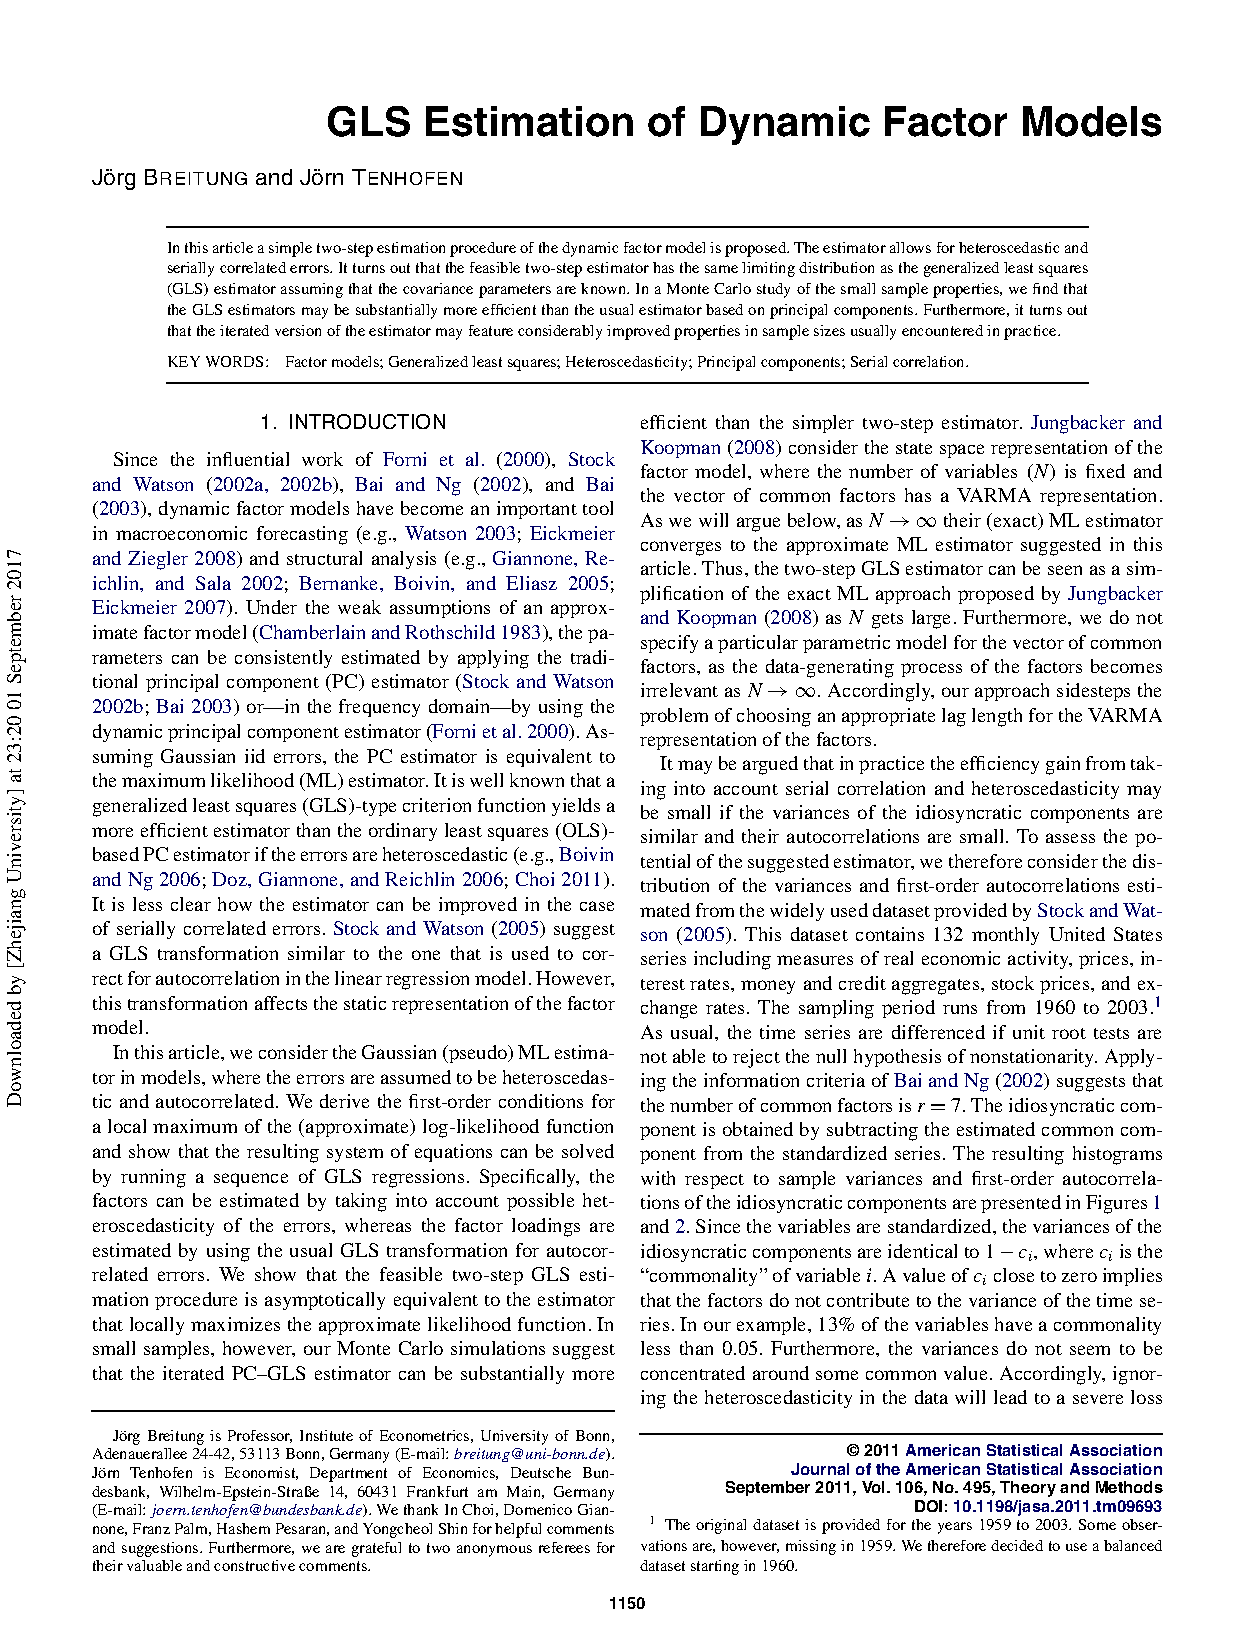
\includepdf[scale=0.9,pages=-,pagecommand={\thispagestyle{followingpage}},addtotoc={
		1, section, 1, Introduction,s1,
		2, section, 1, The Dynamic Factor Model,s2,
		3, section, 1, The PC-GLS Estimator,s3,
		4, section, 1, Asymptotic Distribution of The Two-step PC-GLS Estimator, s4,
		6, section, 1, Asymptotic Efficiency, s5,
		7, section, 1, Small Sample Properties,s6,
		7, subsection, 2, Simulation in a Controlled Environment, s61,
		8, subsubsection, 3, Autocorrelation and Heteroscedasticity, s62,
		9, subsubsection, 3, Introducing Cross-Sectional Correlation, s63,
		10, subsubsection, 3, The Hybrid Estimator, s64,
		11, subsection, 2, Simulation Based on Stock and Watson's (2005) Dataset, s62,
		13, section, 1, Conclusion, s7}]{gls-original-2.pdf}
	\addtocontents{toc}{\protect\contentsline{assess}{\protect\numberline{}浙江大学本科生文献综述和开题报告考核表}{}} % just combine

\end{document}